%1. Common problems and common technologies [+]
% - Text search +
% - Self Index +
% - Problems with self indexation +
% - Full text search with substrings +
%2. SA: overview, complexity, usage         [+]
%3. Radix: overview, complexity, usage      [+]
%4. Succinct data                           [+]
%5. CSA                                     [+]
%6. PSI                                     [+]
%7. Regenerating SA from PSI                [+]
%8. EF                                      [+]
%9. My CSA                                  []
%10.Complexity                              []

\textbf{Text retrieval}

Currently the Internet is updated with a large amount of data everyday.
That is why it is extremely important to organize search of necessary information in an \emph{effective} way.
In search within document indexing is applied.
\emph{Inverted index} is traditional for text indexing.
It is a data structure in which for each word in a document collection corresponding list
contains all the documents of a collection where this word is present.
While processing a multiple word request the intersection of lists is used,
that is corresponded to each word in a query.

\textbf{Problems of traditional approaches}

Some cases take place in practice where it is impossible to use
traditional full-text search by words \cite{bast2013efficient}.
A search model in which the task is to find orthographically close words (\emph{fuzzy search}),
that is used for spelling correction in numerous text editors,
does not allow one to solve the problem using full-text search.
The same applies to different systems where \emph{pattern matching} is used \cite{bai2018adaptive}.
Another example of texts where it is difficult to apply traditional search method
are several eastern languages.
In these languages words are not separated by spaces that makes \emph{inverted index} difficult to use.
Finally large texts combined from alphabet with a small amount of symbols can be attributed to <<inconvenient>> texts.
A typical example of these texts is DNA and protein structure code.
This text is not separated on words that is a key issue in using \emph{inverted index}.

To solve these problems it is necessary to perform substring search.
Existing methods (prefix tree, suffix array) take too much space therefore they are not effective.
For example, prefix tree that contains \emph{n} words with $C$ average number of symbols in a word
takes $O(n \cdot C)$ memory \cite{aho1975efficient}.
Let's take a greater look at suffix array as one of the most popular textual information indexation methods.

\textbf{Полнотекстовый поиск при помощи suffix array}

Suffix array -- это структура данных, используемая в полнотекстовой индексации, позволяющая выполнять
поиск подстроки в тексте размером n символов за $O(\log{}n)$ \cite{manber1993suffix}.
При этом для хранения n слов в suffix array необходимо $O(n \log{}n)$ памяти.
Так для ASCII-текста размером $2^{32}$ требуется $2^{32} \cdot 8 = 32$ гигабит пространства памяти.
Для такого текста suffix array должен содержать элементы размером 32 бита.
Тогда размер suffix array достигает $2^{32} \cdot 32 = 128$ гигабит пространства памяти,
что в 4 раза превышает размер исходного текста.

Suffix array представляет собой отсортированную в лексикографическом порядке
последовательность суффиксов. Для лучшего понимания устройства suffix array, рассмотрим эту структуру данных на примере индексирования
слова mississippi:
\\(0) mississippi
\\(1) ississippi
\\(2) ssissippi
\\(3) sissippi
\\(4) issippi
\\(5) ssippi
\\(6) sippi
\\(7) ippi
\\(8) ppi
\\(9) pi
\\(10) i

Suffix array, составленный из таких суффиксов, будет иметь вид:

10 7 4 1 0 9 8 6 3 5 2

Обычно конец документа обозначается специальным символом, не входящим в алфавит хранящегося в массиве текста.
В качестве такого разделителя в этой работе был выбран символ доллара \$.
Современные подходы по построению suffix array позволяют конструировать структуру данных за $O(n)$.

\textbf{Radix tree}

% Picture By Claudio Rocchini - Own work, CC BY 2.5, https://commons.wikimedia.org/w/index.php?curid=2118795

\begin{wrapfigure}{r}{0.25\textwidth} %this figure will be at the right
 \centering
 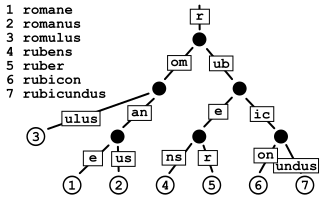
\includegraphics[width=0.45\textwidth]{PatriciaTrie}
 \caption{Пример Radix tree}
\end{wrapfigure}

Radix tree представляет собой сжатое prefix tree. В свою очередь, prefix tree является
структурой данных, которая предоставляет интерфейс ассоциативного массива и позволяет
хранить значения в виде key-value пар.
В этом исследовании в качестве key выбраны строки, причем в отличие от обычный деревьев,
на ребрах radix tree могут храниться как один элемент (символ),
так и последовательность элементов (строка).

Radix tree широко применяется в ядре Linux для связи указателя с длинным целочисленным ключом \cite{Linux2018}.
Эта структура данных эффективна с точки зрения скорости поиска и хранения информации.
В то же время, Radix tree применяется в IP-адресации, так как очень удобна для хранения
иерархической структуры IP-адресов \cite{Radix2019}.

Рассмотрим подробнее характеристики radix tree. Пусть требуется хранить ключи размером k
при хранении n элементов в дереве. Тогда добавление элемента, поиск и удаление элемента
занимают $O(k)$ операций \cite{leis2013adaptive}.

Для многих запросов поиска по словарю radix tree может быть быстрее и эффективнее, чем хеш-таблицы.
Несмотря на то, что обычно сложность поиска по хэш таблице принимают за $O(1)$,
при этом игнорируется необходимость сначала хешировать входные данные.
На это обычно требуется $O(k)$ операций, где k -- длина входной строки.
Radix tree выполняет поиск за $O(k)$, без необходимости сначала хешировать и имеют гораздо лучшую локальность кеша.
Они также сохраняют порядок, позволяя выполнять упорядоченное сканирование,
получать минимальные / максимальные значения, сканировать по общему префиксу и т.д.

Благодаря всем этим преимуществам, radix tree широко распространено в базе данных Redis, программных продуктах
компании HashiCorp, таких как Terraform, Consul, Vault, Nomad и т.д. \cite{Redis2018},
что представляет дополнительный интерес для его изучения на текстовых данных и сравнения с suffix array.

\textbf{Сжатое представление данных}

Одной из главных задач этой работы является программная реализация сжатого хранения индекса для suffix array.
Поэтому важно определить, какие данные можно считать сжатыми.

Существуют различные степени сжатости информации.
Предположим, что для хранения некоторого количества данных требуется Z бит.
Сжатые (succinct) структуры данных занимают \(Z + o(Z)\) бит, implicit -- \(Z + o(1)\) бит и
compact -- \(O(Z)\)) бит \cite{huo2014practical}. В этой работе предлагается сжать suffix array, представив его в succinct виде.
Таким образом, размер массива немногих больше превосходит размер исходного текста.

\textbf{$\Psi$-массив}

Важным место в теории сжатого представления индекса занимает промежуточный $\psi$-массив.
Характерной особенностью всех алгоритмов сжатия succinct suffix array (CSA)
является то, что сжимается не непосредственно индекс, а его представление
в виде $\psi$-массива. Вспомогательный массив можно получить из suffix array путем следующих манипуляций с индексами.
\newpage
Рассмотрим построение $\psi$-массива на примере знакомой строки \textbf{mississippi\$}:
\\ \textbf{Text}:\,\,\,\,\,\,\,\,\,\,\,\,\,\,\,\,\,\,\,\,\,\,\,\, m \,i \,\,\,\,s \,\,\,s \,\,\,\,i \,\,\,\,s \,\,\,s \,\,i \,\,p \,\,p \,\,i \,\,\,\,\$
\\ \textbf{Offset}:\,\,\,\,\,\,\,\,\,\,\,\,\,\,\,\,\,\,\,\, 0 \,\,1 \,\,\,\,2 \,\,3 \,\,\,4 \,\,\,5 \,\,6 \,7 \,\,8 \,\,9 \,10 11
\\ \textbf{Suffix Array}:   11 10 \,7 \,\,4 \,\,\,1 \,\,\,0 \,\,9 \,8 \,\,6 \,\,3 \,\,5 \,\,2
\\ \textbf{$\Psi$ -array}: \,\,\,\,\,\,\,\,\,\,\,\,\$ \,\,\,0 \,\,\,\,7 10 \,\,11 4 \,\,1 \,6 \,\,2 \,\,3 \,\,8 \,\,9

Будем называть потомком (successor) самый большой суффикс подстроки, кроме исходной подстроки.
Т.е. для подстроки issippi\$ потомком является ssippi\$.
$\Psi$-массив указывает на потомок для каждого выбранного суффикса.
Например, рассмотрим $SA[7] = 8$. Его потомком является позиция в suffix array, которая хранит $8 + 1 = 9$.
Таким образом, $\psi[7] = 6$. Главное соотношение между $\Psi$-массивом и suffix array:
\begin{equation}\label{sa:1}
 SA[i] = SA[\psi[i]] - 1
\end{equation}
Необходимо отметить, что $\Psi[0] = \$$, т.к. для первого элемента в suffix array нет потомка.
При этом $SA[5]$ ссылается на 0-й индекс, то есть на всю строку целиком.
Иными словами, элемент suffix array ссылается на начало текста,
т.е. никакой другой суффикс не может иметь его в качестве потомка.
Соответственно в $\psi$-массиве нет элемента, равного 5.

\textbf{Восстановление suffix array из $\psi$-массива}

Существует возможность восстановить исходный suffix array по сгенерированному $\psi$-массиву
фактически с помощью операций, обратных к тем, которые были представлены в предыдущем параграфе.
Коснемся подробнее особенностей работы этого алгоритма.

В первую очередь необходимо найти индекс элемента suffix array, который не встречается в $\psi$-массиве.
В нашем примере он равен 5. Из приведенных выше рассуждений следует, что $SA[5] = 0$.
Таким образом был декодирован один элемент исходного suffix array. Из формулы \ref{sa:1} для $i = 5$ следует:

\[SA[5] = SA[\psi[5]] - 1\]
\[0 = SA[4] - 1\]
\[SA[4] = 1\]

Еще один элемент suffix array восстановлен! Таким образом можно восстановить всю оставшуюся последовательность.
Время на поиск первого элемента составляет \(O(n)\) операций.
Существуют некоторые улучшения скорости поиска нужного элемента в suffix array, требующие дополнительных
структур данных, хранящих значение suffix array на каждом \(\log n\) шаге \cite{andersensimple}.
Такой способ выходит за рамки этой работы, поскольку главной задачей является максимальное сжатие индекса.

\textbf{Сжатие $\psi$-массива}

Рассмотрим подробнее $\psi$-массив:
\\ \textbf{Text}:\,\,\,\,\,\,\,\,\,\,\,\,\,\,\,\,\,\,\,\,\,\,\,\, m \,i \,\,\,\,s \,\,\,s \,\,\,\,i \,\,\,\,s \,\,\,s \,\,i \,\,p \,\,p \,\,i \,\,\,\,\$
\\ \textbf{Offset}:\,\,\,\,\,\,\,\,\,\,\,\,\,\,\,\,\,\,\,\, 0 \,\,1 \,\,\,\,2 \,\,3 \,\,\,4 \,\,\,5 \,\,6 \,7 \,\,8 \,\,9 \,10 11
\\ \textbf{Suffix Array}:   11 10 \,7 \,\,4 \,\,\,1 \,\,\,0 \,\,9 \,8 \,\,6 \,\,3 \,\,5 \,\,2
\\ \textbf{$\Psi$ -array}: \,\,\,\,\,\,\,\,\,\,\,\,\$ \,\,\,0 \,\,\,\,7 10 \,\,11 4 \,\,1 \,6 \,\,2 \,\,3 \,\,8 \,\,9

Отсортированный набор суффиксов имеет вид:
\\ (0) \,\,\,\$
\\ (1) \,\,\,i\$
\\ (2) \,\,\,ippi\$
\\ (3) \,\,\,issippi\$
\\ (4) \,\,\,ississippi\$
\\ (5) \,\,\,mississippi\$
\\ (6) \,\,\,pi\$
\\ (7) \,\,\,ppi\$
\\ (8) \,\,\,sippi\$
\\ (9) \,\,\,sissippi\$
\\ (10) ssippi\$
\\ (11) ssissippi\$

Стоит обратить внимание на его структуру: он состоит из набора возрастающих последовательностей индексов.
Рассмотрим возрастающую последовательность 2, 3, 8, 9.

$SA[2] = 7$, $T[7] = i$.
$SA[3] = 4$, $T[4] = i$. Примечательно, что $SA[6] = 9$, $T[9] = p$.
То есть чередование индексов с возрастания на убывание соответствует смене символа с i на p.

\begin{theorem}
 \label{lemma:1}
 Два последовательных элемента $\psi$-массива являются возрастающими, если соответствующие суффиксы,
 на которые они ссылаются, начинаются с одного и того же символа.
\end{theorem}

\begin{proof}
 По построению, suffix array представляет собой набор индексов в исходном тексте,
 отсортированный в лексикографическом порядке. Это означает, что $T[SA[i]] < T[SA[i + 1]]$
 $\forall i \in [0, n).$ Эти два суффикса имеют общий первый символ. Поэтому они отличаются в следующих
 элементах, например, во втором: $T[SA[i] + 1] < T[SA[i + 1] + 1].$

 $\Psi$-массив ссылается на потомка для данного суффикса: $T[SA[\psi[i]]] < T[SA[i] + 1].$
 Т.к. $T[SA[i]]$ и $T[SA[i + 1]]$ имеют одинаковый первый символ, их потомки упорядочены.
 Если $T[SA[\psi[i]]] < T[SA[\psi[i + 1]]]$, тогда из-за упорядоченности индекс в suffix array
 для первого должен находиться перед индексом для второго. Следовательно индексы (значения $\psi$-массива)
 должны быть упорядочены, если суффиксы имеют общий первый символ.
\end{proof}

Возрастающие последовательности неотрицательных целых чисел сжимаемы \cite{andersensimple}.
Самый простой путь для хранения таких последовательностей -- битмап.
Однако этот способ не позволяет иметь произвольный доступ к элементам.
Рассмотрим более совершенный алгоритм сжатого представления данных.

\textbf{Кодировка Elias--Fano}

Сжатие при помощи метода Elias--Fano \cite{pibiri2014dynamic}
позволяет представлять монотонно возрастающие последовательности
целых неотрицательных чисел в виде битовых векторов. Этот способ делает возможным
хранение неубывающей последовательности $n$ целых чисел размером $[0, m)$,
занимая $2n + n[\log m/n]$ бит, предоставляя доступ к $i$-му элементу за $O(1)$.
Сравнив размеры структуры данных с минимально возможным занимаемым местом в памяти
с точки зрения теории информации, Elias--Fano кодировка является сжатым (succinct) индексом.

\begin{figure}[t]
 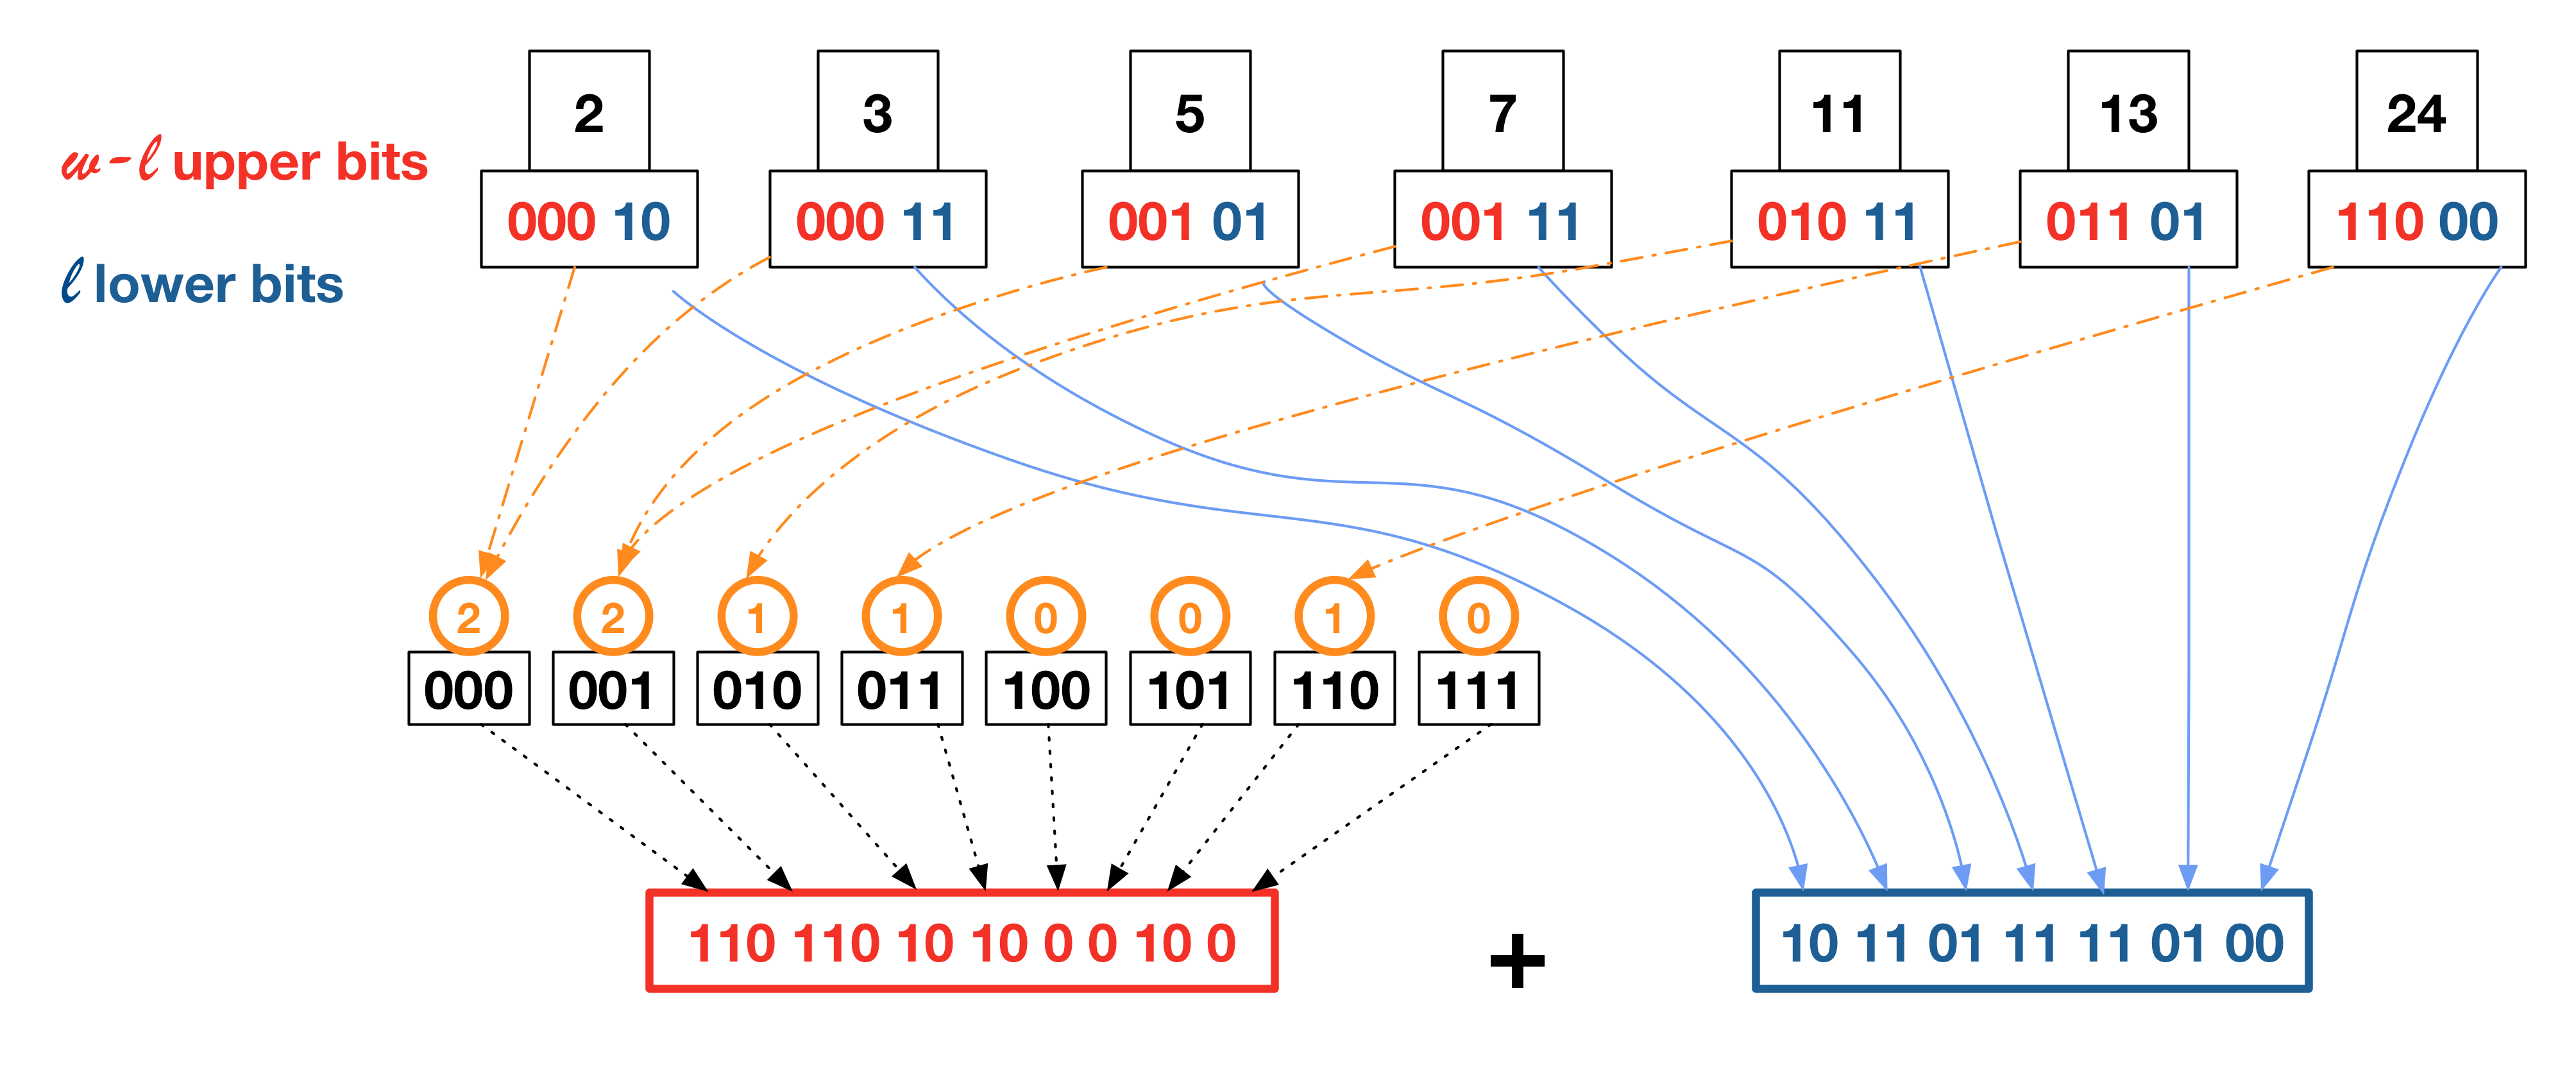
\includegraphics[width=12cm]{Elias-Fano}
 \caption{Пример построения кода Elias-Fano}
 \centering
 \label{fig:EF}
\end{figure}

В начале каждое число из последовательности кодируется $\log m$ битами данных.
Двоичное представление элементов разбито на две части: верхнюю часть, содержащую в себе
первые $\log n$ бит, и нижнюю, с оставшимися $\log m - \log n = \log m / n$ бит.
Объединение нижних битов занимает $n \log m$ бит. Верхние биты представляют собой
набор из $n + m / 2^{\log m/n}$ бит \cite{antonio2018integers}.
Начиная с пустого битового вектора, мы добавляем в эту часть 0
в качестве стоп-бита для каждого возможного значения, представляемого битами старшей части.
Мы добавляем 1 для каждого фактически присутствующего значения, выставляя его перед соответствующим стоп-битом.

В качестве примера рассмотрим отсортированную последовательность {2,3,5,7,11,13,24}.
На рисунке \ref{fig:EF} показана схема кодирования. Наибольшим числом в наборе (universe) является 24.
Поэтому для представления каждого элемента необходимо выделить 5 бит на элемент.
Затем нужно разбить бинарное представление на две части: верхнюю и нижнюю.
Исходя из ранее оговоренных условий, выберем 3 бита под верхнюю часть и 2 бита под нижнюю.
Всего в последовательности присутствует 7 элементов. Рассмотрим число 2. Для него имеем
$2 = 0b00010$ и соответственно 000 в качестве верхней части и 10 в качестве нижней.
Повторяя этот процесс, получим набор нижних частей для каждого элемента.
Затем объединим полученные части вместе. Для верхних частей имеется $2^3$ вариантов
наборов значений. С каждым таким набором ассоциируется счетчик, который увеличивается на единицу,
если число из последовательности имеет соответствующую верхнюю часть.
Так для 2 инкрементируем набор 000. Число $3 = 0b00011$ с верхней частью 000 идет в тот же набор.
Для числа $5 = 0b00101$ с верхней частью 001 инкрементируем набор 001 и т.д.
Наконец, кодируем счетчики унарно, добавляя столько единиц в представление счетчика,
сколько имеет значение каждого счетчика, за которым следует 0 бит.
Окончательное кодирование Elias-Fano получается объединением полученных верхней и нижней частей.

\textbf{Восстановление данных из кода Elias--Fano}

Для восстановления исходной монотонной неубывающей последовательности чисел, необходимо разработать операцию
доступа к $i$-му элементу последовательности, $i \in [0, n)$. Для доступа к нижней части
достаточно просто получить соответствующие биты, т.к. длина вектора для хранения элемента известна.
Для получения старшей части, необходимо осуществить операцию \emph{select}.
Операция \emph{select($i$)} позволяет получить позицию $i$-го бита, выставленного в 1 в битовом векторе.
Эта операция может быть выполнена за $O(1)$, что позволяет получать произвольный доступ к элементу
последовательности без полного раскодирования всей последовательности целиком \cite{farina2009rank}.